\documentclass[crop]{standalone}
\usepackage{amssymb}
\usepackage{amsmath}
\usepackage{amsfonts}
\usepackage{color}
\usepackage{tikz}
\usetikzlibrary{math}

\begin{document}
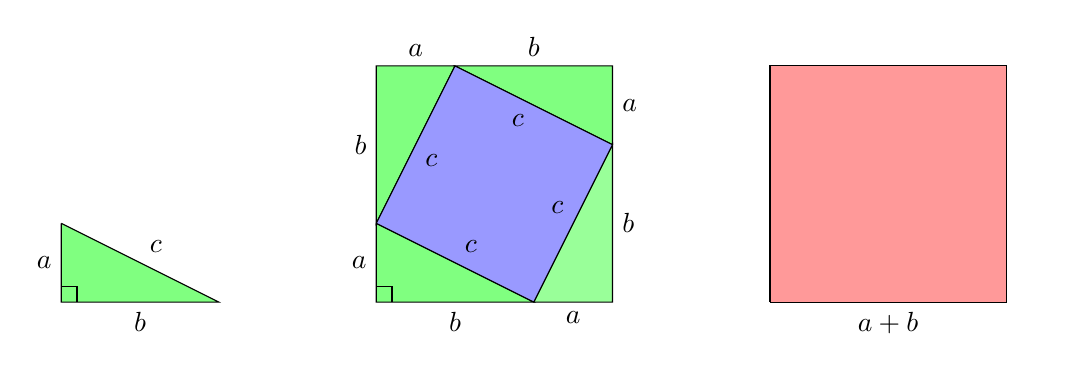
\begin{tikzpicture}
    
    \draw[fill=green!50] (0,1)--(0,0) node[pos=0.5,left]{$a$}--(2,0)node[pos=0.5,below] {$b$} --(0,1)node[pos=0.5,above right]{$c$};
    \draw (0,0.2)-|(0.2,0);

    \tikzmath{\x=4;}
    
    \draw[fill=green!50] (\x,1)--(\x,0) node[pos=0.5,left]{$a$}--(\x+2,0)node[pos=0.5,below] {$b$} --(\x,1);
    \draw (\x,0.2)-|(\x+0.2,0);

    \draw[fill=green!50] (\x+1,3)--(\x,3)node[pos=0.5,above]{$a$}--(\x,1)node[pos=0.5,left]{$b$}--(\x+1,3);
    \draw[fill=green!50] (\x+3,2)--(\x+3,3)node[pos=0.5,right]{$a$}--(\x+1,3)node[pos=0.5,above]{$b$}--(\x+3,2);
    \draw[fill=green!40] (\x+2,0)--(\x+3,0)node[pos=0.5,below]{$a$}--(\x+3,2)node[pos=0.5,right]{$b$}--(\x+2,0);

    \draw[fill=blue!40] (\x,1)--(\x+1,3)node[pos=0.5,below right] {$c$}--(\x+3,2)node[pos=0.5,below left] {$c$}--(\x+2,0)node[pos=0.5,above left] {$c$}--(\x,1)node[pos=0.5,above right] {$c$};

    \tikzmath{\x=9;}
    \draw[fill=red!40] (\x,0)--(\x+3,0) node[pos=0.5,below]{$a+b$}--(\x+3,3)--(\x,3)--(\x,0);    
    \node at (12.5,0) {};    
    
\end{tikzpicture}
\end{document}